\section{Simulation Analysis}
\label{sec:simulation}
In this section we will describe the steps needed to simulate this circuit using the software Ngspice. Three types of analysis will be performed: Operating Point analysis, Transient analysis ans Frequency analysis.

The following steps in the simulations are to be conducted: 
\begin{itemize}
	\item for $t<0$ (operating point only, in order to obtain the voltages in all nodes and the currents in all branches);
	\item operating point for  $V_s(0) = 0$, replacing the capacitor with a a voltage source $V_x = V_6-V_8$, where $V_6$ and $V_8$ are the voltages in nodes 6 and 8 as obtained in the previous step (this step is necessary given that we must the compute the boundary conditions that guarantee continuity in the capacitor's discharge - such may imply that the boundary conditions differ from those computed for $t<0$);
	\item simulate the natural response of the circuit (using the boundary conditions V(6) and V(8) as obtained previously) using a transient analysis;
	\item repeating the third step, using {\it $V_s$} as given in \textbf{Figure~\ref{fig:time_step}} and f = 1kHz  in order to simulate for the total response on node 6
	\item simulate the frequency response in node 6 for a frequency range 0.1 Hz to 1MHz.
\end{itemize}
 
 \begin{figure}[H] \centering
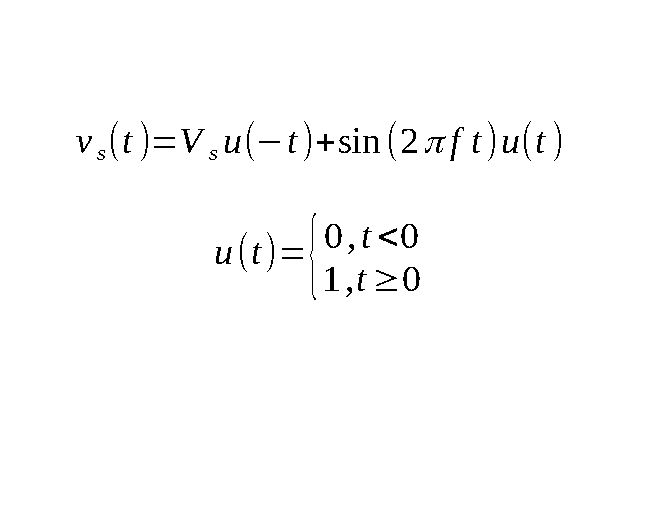
\includegraphics[width=0.5\linewidth]{time_step.pdf}
\caption{Time step conditions}
\label{fig:time_step}
\end{figure}

%ponto 1
\subsection{Operating Point Analysis for $t<0$}
There was a need to create a "fictional" voltage source, between node 7 and resistor 6 (providing 0V to the circuit in order not to alter the behaviour of the rest of the circuit) so as to be able to define the dependecy for the current-controlled voltage source {\it $V_d$}. This has no specific reason to be, other than the particularities of the Ngspice software. The circuit and nodes used for the simulation can be seen in \textbf{Figure~\ref{fig:diagram_t2}}.\par 
\textbf{Table~\ref{tab:op}} shows the simulated operating point results for the circuit
under analysis for $t<0$. 
%The current flows considered in the theoretical section were coherent with the polarity implicitly declared when defining the circuit to be simulated in the Ngspice script.\par

\begin{table}[h!]
  \centering
  \begin{tabular}{|l|r|}
    \hline    
    {\bf Name} & {\bf Value [mA or V]} \\ \hline
    @c[i] & 0.000000e+00\\ \hline
@gb[i] & -2.91567e-04\\ \hline
@r1[i] & 2.780494e-04\\ \hline
@r2[i] & 2.915672e-04\\ \hline
@r3[i] & -1.35178e-05\\ \hline
@r4[i] & -1.22689e-03\\ \hline
@r5[i] & -2.91567e-04\\ \hline
@r6[i] & 9.488377e-04\\ \hline
@r7[i] & 9.488377e-04\\ \hline
v(1) & 5.243596e+00\\ \hline
v(2) & 4.952739e+00\\ \hline
v(3) & 4.367468e+00\\ \hline
v(4) & -1.96340e+00\\ \hline
v(5) & 4.994112e+00\\ \hline
v(6) & 5.904536e+00\\ \hline
v(7) & -1.96340e+00\\ \hline
v(8) & -2.92677e+00\\ \hline

  \end{tabular}
  \caption{Operating point for $t<0$. A variable preceded by @ is of type {\em current}
    and expressed in miliAmpere; other variables are of type {\it voltage} and expressed in
    Volt.}
  \label{tab:op}
\end{table}

%ponto 2
\pagebreak
\subsection{Operating Point Analysis for $t=0$}
In this section the circuit was simulated using an operating point analysis with $V_s(0) = 0$ and 
with the capacitor replaced by a voltage source {\it $V_x=V(6)-V(8)$} with these as obtained in the last step. This step was taken because we must compute the boundary conditions that guarantee continuity in the capacitor's discharge (such may imply that the boundary conditions differ from those computed for $t<0$). In other words $V(6)-V(8)$ needs to be a continuos function in time (in this case particularly from $t<0$ to $t=0$), as there can not be a energy discontinuity in the capacitor ($E_C=\frac{1}{2}CV^{2}$). However, that does not imply that that $V(6)$ and $V(8)$ are continuos functions in time.
In \textbf{Table~\ref{tab:opeq}} the simulation results are presented. 
\begin{table}[h!]
  \centering
  \begin{tabular}{|l|r|}
    \hline    
    {\bf Name} & {\bf Value [mA or V and Ohm]} \\ \hline
    @gb[i] & 4.151983e-18\\ \hline
@r1[i] & -3.95949e-18\\ \hline
@r2[i] & -4.15198e-18\\ \hline
@r3[i] & 1.924970e-19\\ \hline
@r4[i] & -8.72784e-19\\ \hline
@r5[i] & -2.82826e-03\\ \hline
@r6[i] & 4.336809e-19\\ \hline
@r7[i] & -8.83871e-19\\ \hline
v(1) & 0.000000e+00\\ \hline
v(2) & 4.141871e-15\\ \hline
v(3) & 1.247625e-14\\ \hline
v(4) & -8.97403e-16\\ \hline
v(5) & 3.552714e-15\\ \hline
v(6) & 8.831302e+00\\ \hline
v(7) & -8.97403e-16\\ \hline
v(8) & 0.000000e+00\\ \hline
Ix & -2.82826e-03\\ \hline
Vx & 8.831302e+00\\ \hline
Req & -3.12252e+03\\ \hline

  \end{tabular} 
  \caption{Operating point for {\it $v_s(0)=0$}. A variable preceded by @ is of type {\em current}
    and expressed in miliAmpere; variables are of type {\it voltage} and expressed in
    Volt. The equivalent resistance is in Ohms}
  \label{tab:opeq}
\end{table}

\pagebreak
%ponto 3
 
\subsection{ Natural solution for $V_6$ using transient analysis}
In this section the natural response of the circuit in the interval [0,20] ms was studied using a transient analysis simulation. To do so the boundary conditions V(6) and V(8) obtained in the previous section were used, as well as the NgSpice directive \textit{.ic}. These values are being obtained from the previous simulations run, and not from the theoretical previsions. 
\par
\begin{figure}[H] \centering
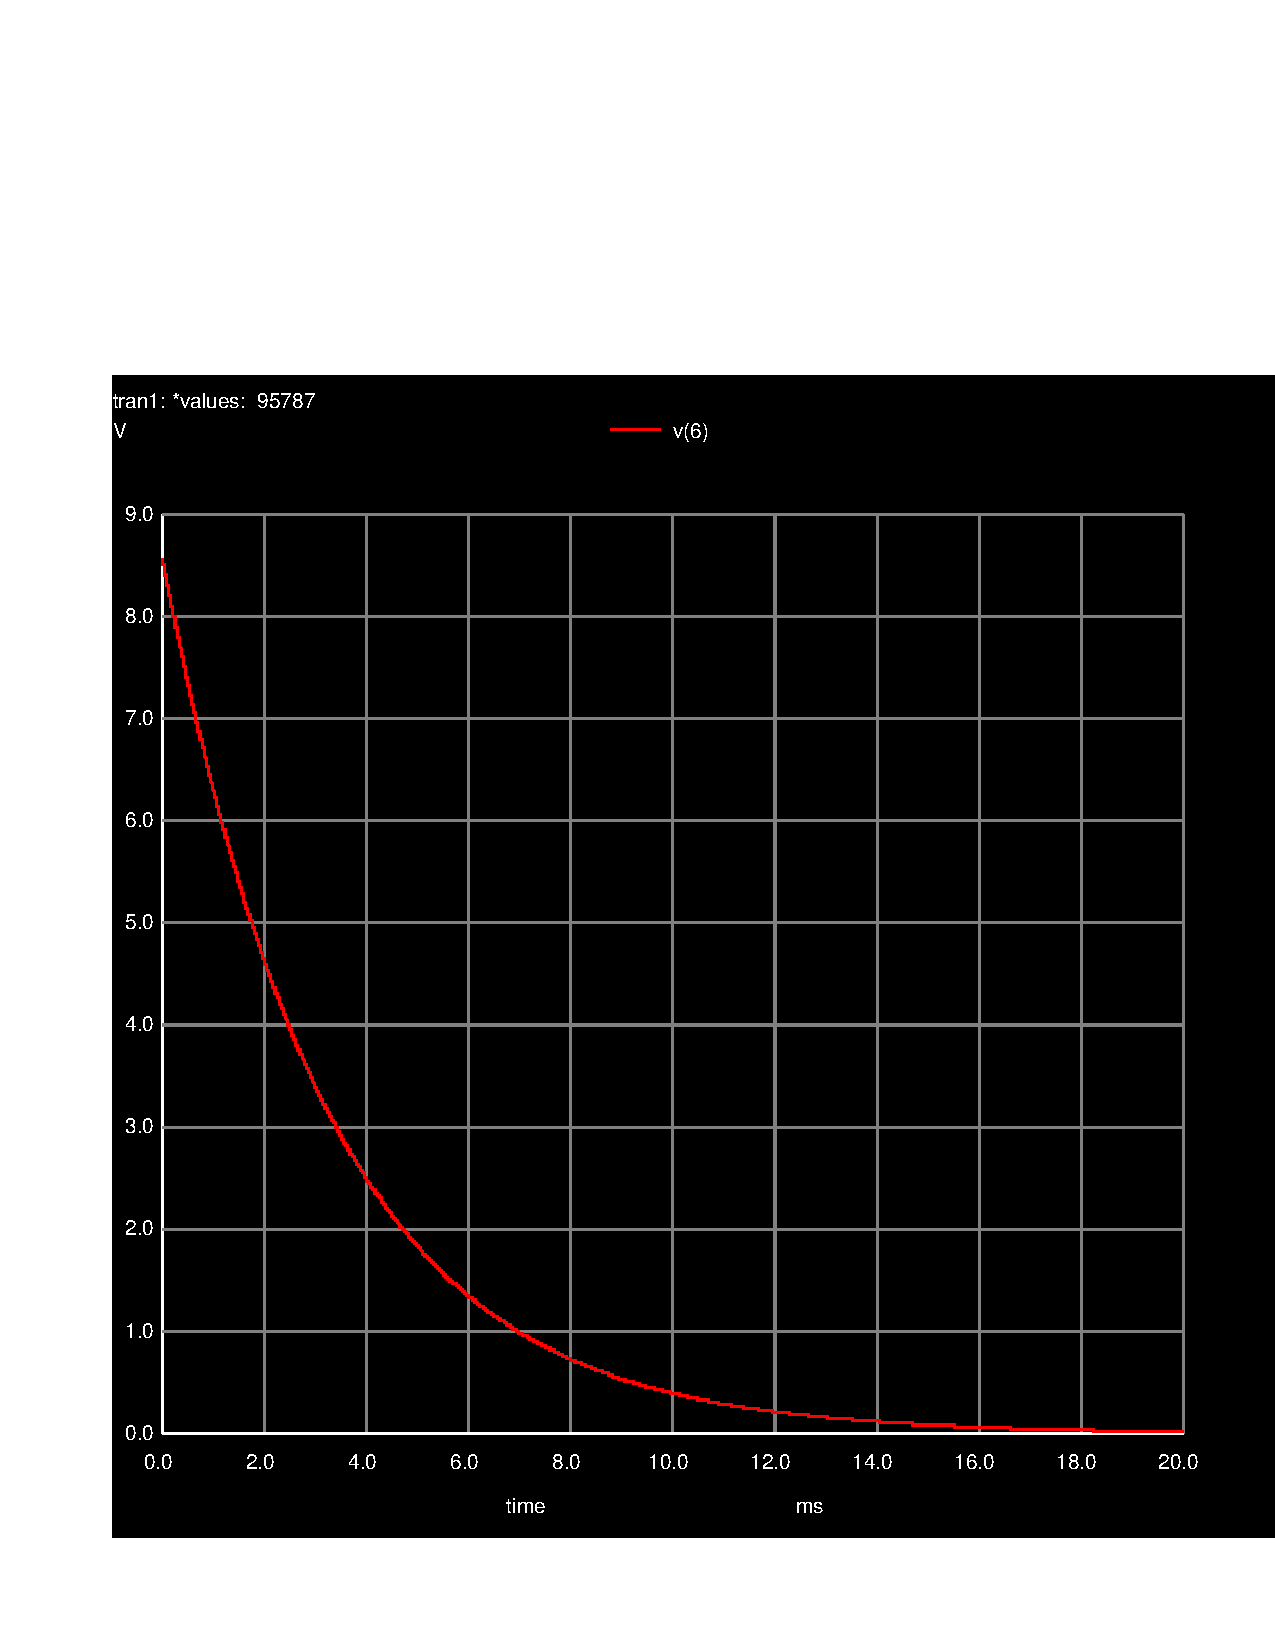
\includegraphics[width=0.6\linewidth]{trans.pdf}
\caption{Simulated natural response of $V_6(t)$ in the interval [0,20] ms. The \textit{x axis} represents the time in miliseconds and the \textit{y axis} the Potencial in node 6  in Volts.  }
\label{fig:transient}
\end{figure}

\pagebreak
%ponto 4
\subsection{ Total solution for $V_6$ using transient analysis}

In this section the total response of $V_6$ (natural + forced) is simulated using transient analysis. This is done by repeating the previous section, but using {\it $V_s$} as given in \textbf{Figure~\ref{fig:time_step}} and f = 1kHz.\par
\begin{figure}[H] \centering
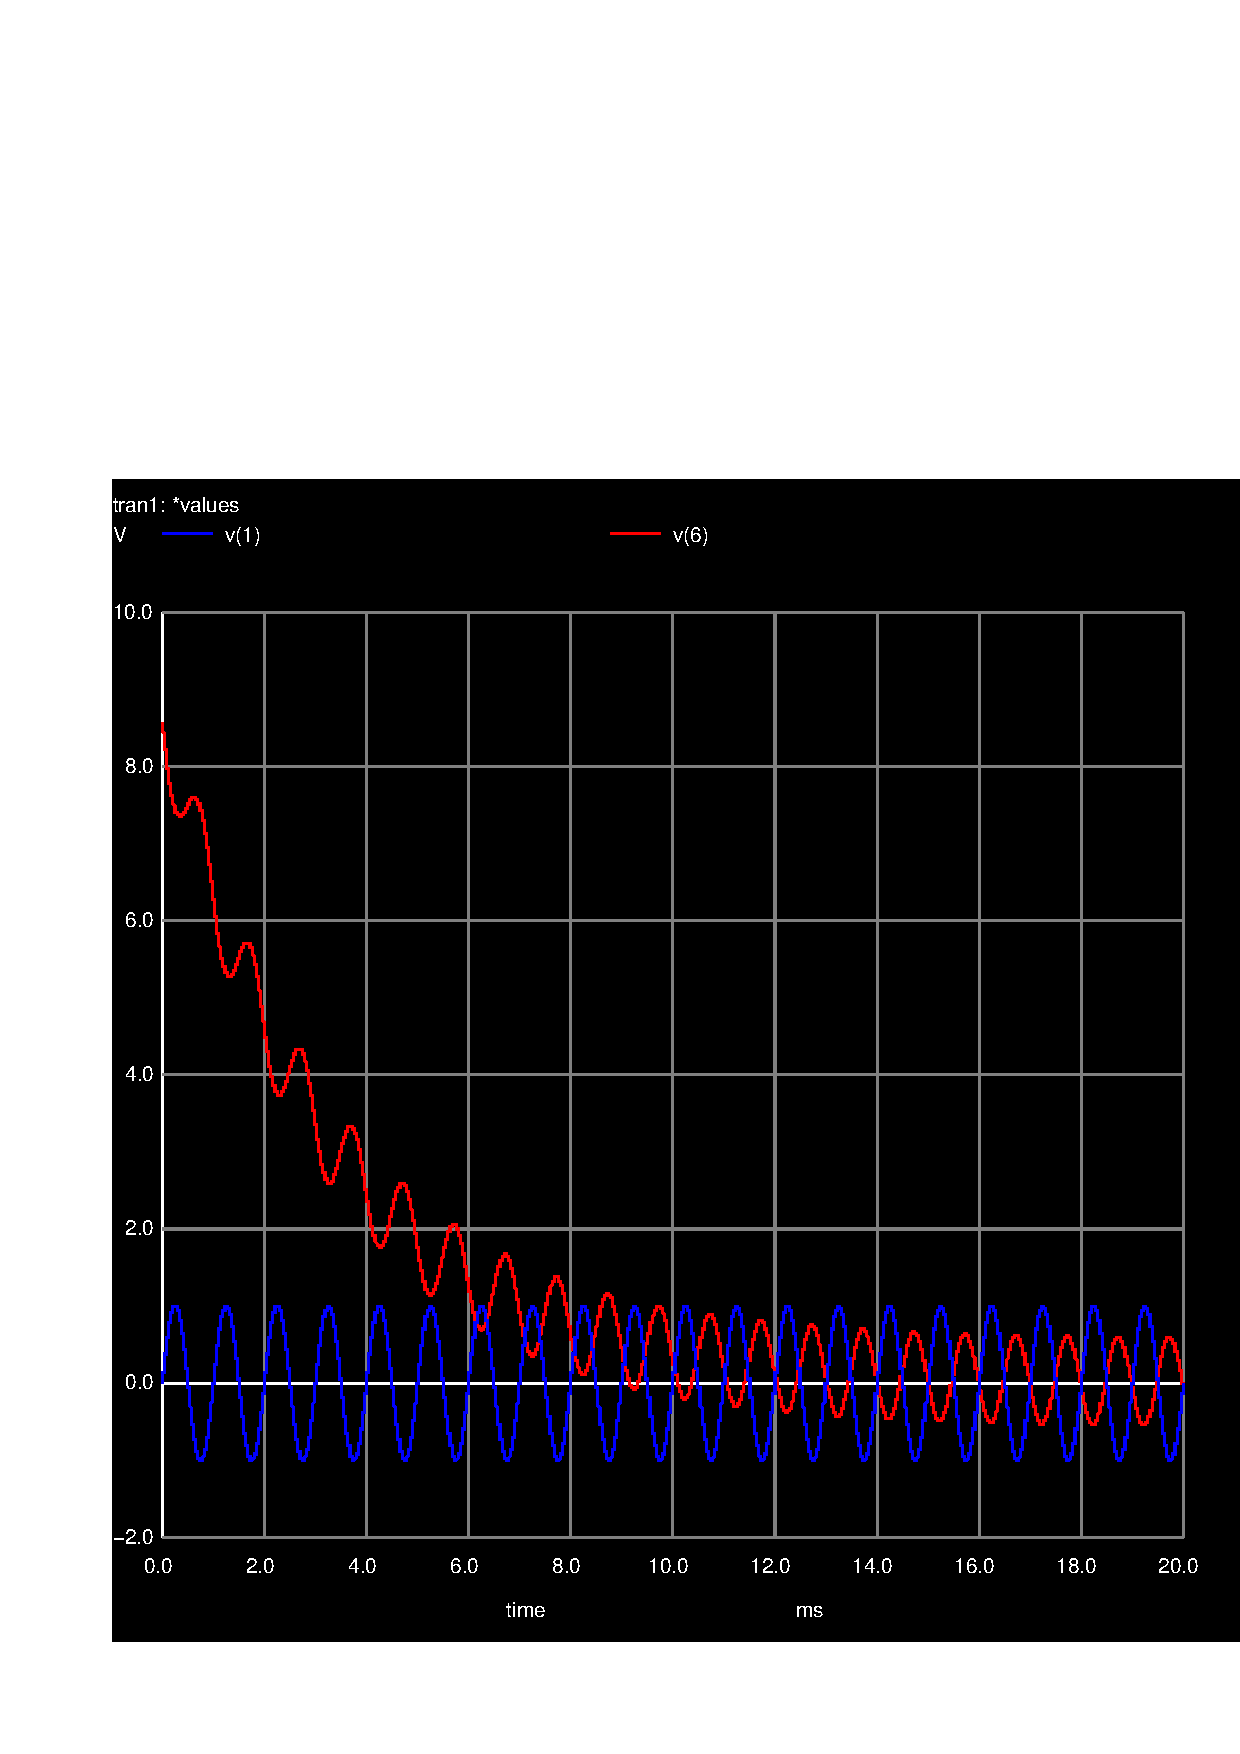
\includegraphics[width=0.6\linewidth]{transv5vs.pdf}
\caption{Simulated response of $V_{6}(t)$ and of the stimulus $V_{s}(t)$ as functions of time from [0,20] ms. The \textit{x axis} represents the time in miliseconds and the \textit{y axis} the Voltage in Volts.}
\label{fig:resp_total}
\end{figure}

%ponto 5
\pagebreak
\subsection{ Frequency response in node 6}
In this section the frequency response in node 6 is simulated for the frequency range from 0.1 Hz to 1 MHz. 
The reasons of how and why $V_{6}(t)$ and $V_{s}(t)$ differ have been coverd in \textbf{subsection ~\ref{ref}}.\par
\begin{figure}[H] \centering
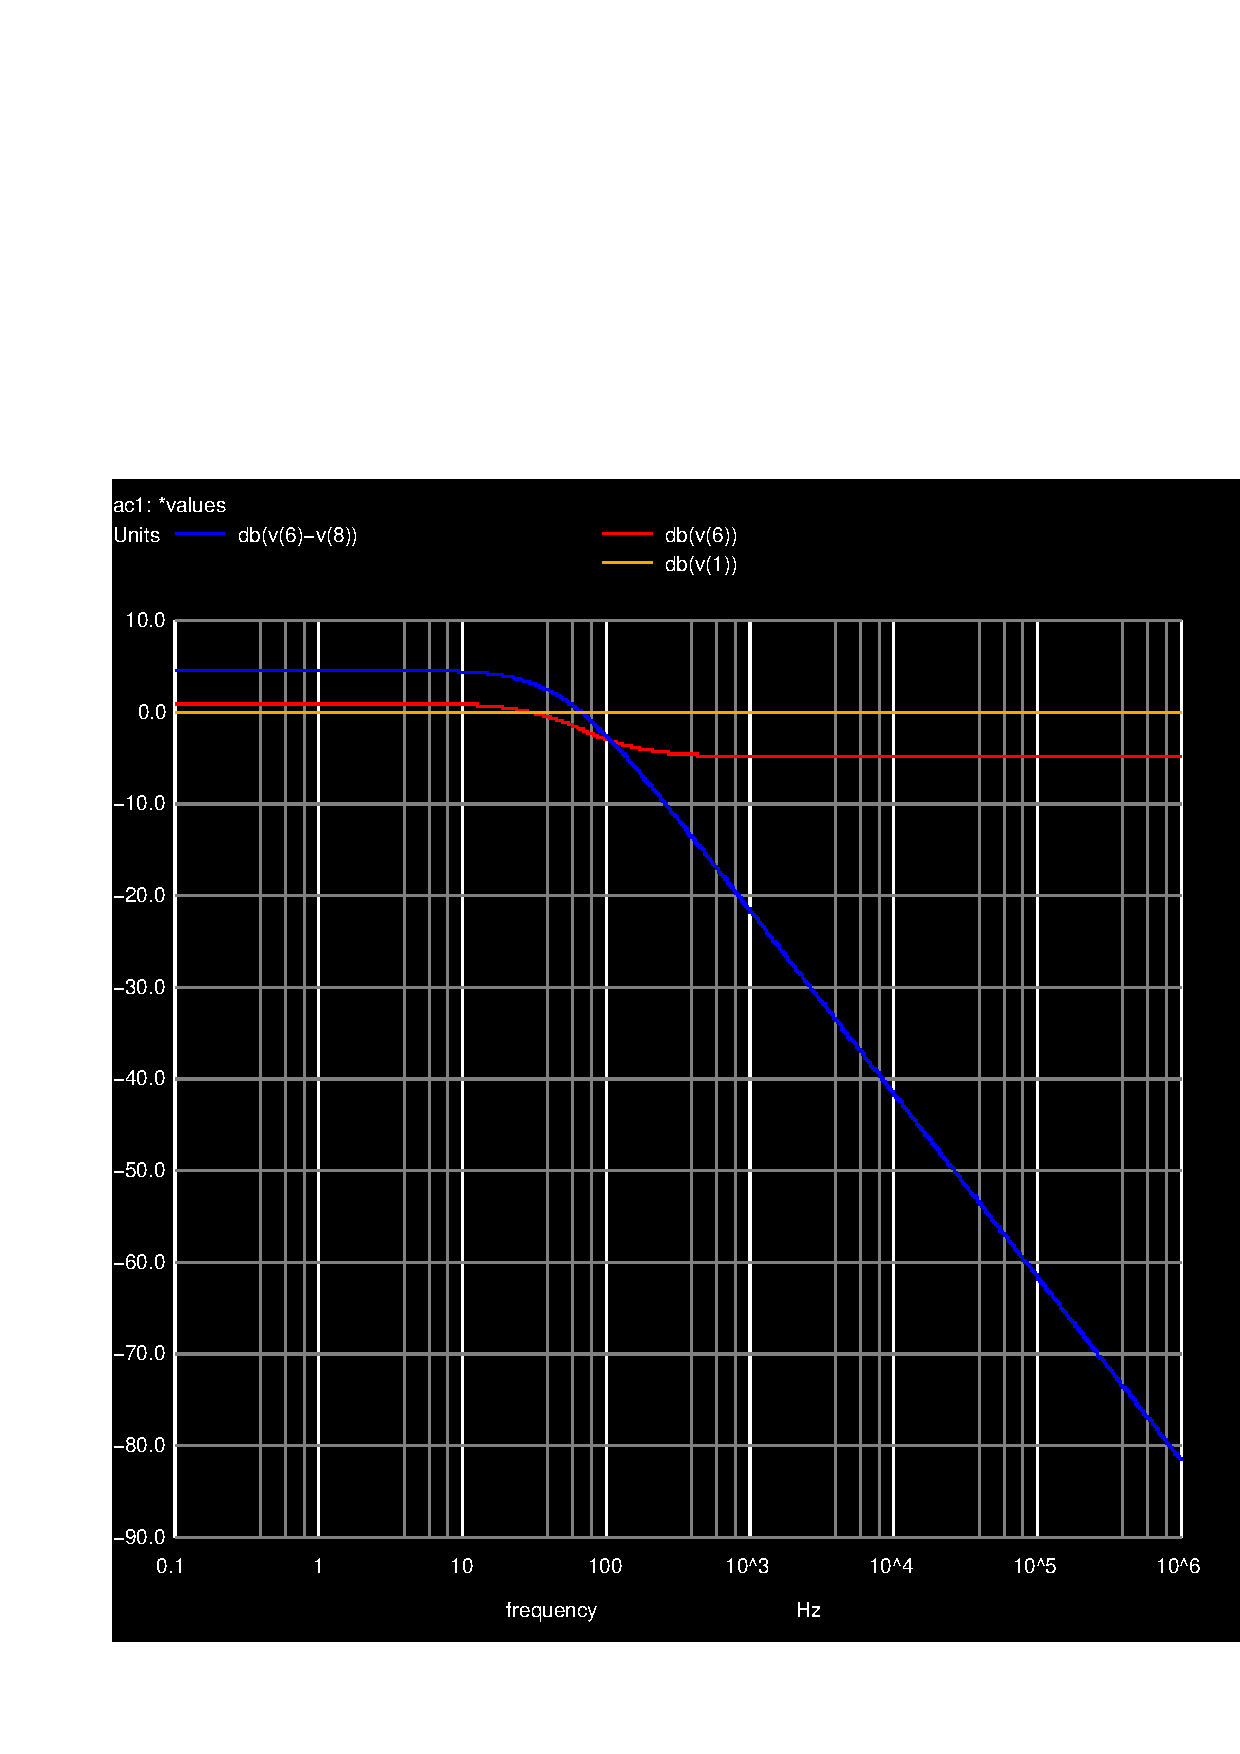
\includegraphics[width=0.6\linewidth]{acm.pdf}
\caption{Magnitude of $V_s(f)$, $V_c(f)$  and of $V_6(f)$. The \textit{x axis} represents the frequency in Hz, using a logarithmic scale and the \textit{y axis} the magnitude in dB.}
\label{fig:Magnitude}
\end{figure}
\pagebreak
\par
\begin{figure}[H] \centering
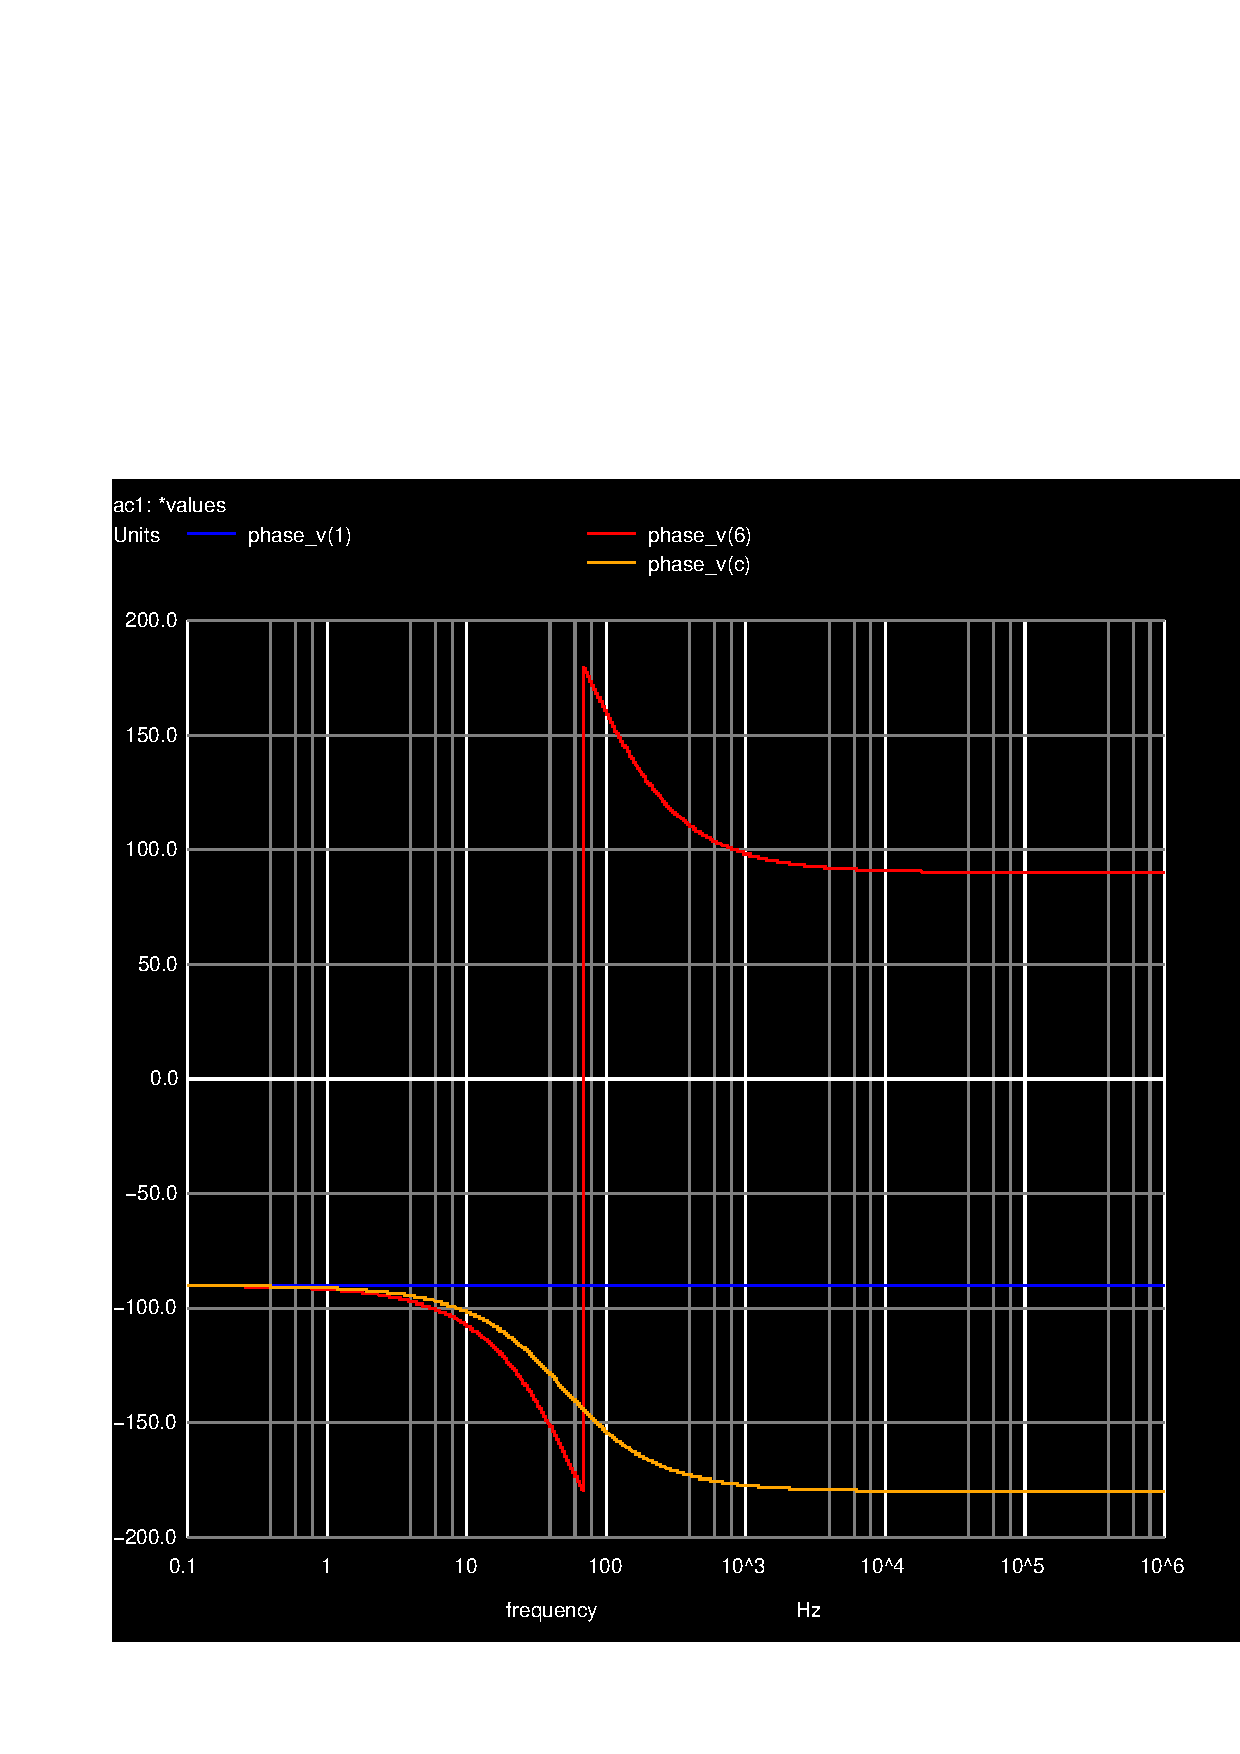
\includegraphics[width=0.6\linewidth]{phase.pdf}
\caption{Phase of $V_s(f)$, $V_c(f)$ and of $V_6(f)$. The \textit{x axis} represents the frequency in HZ, using a logarithmic scale and the \textit{y axis} the phase in degrees.}  
\label{fig:phase}
\end{figure}

\pagebreak
